\documentclass[11pt]{article}
\usepackage[utf8]{inputenc}%
\usepackage[unicode]{hyperref}%
\urlstyle{same}%
\usepackage{url}
\usepackage{multicol}
\usepackage{xcolor}
\usepackage{hyperref}
\usepackage{graphicx}
\usepackage{subcaption}
\usepackage{enumitem}


\title{Multicols Demo}
\renewcommand{\baselinestretch}{1.1}

%%% Add packages here
	\usepackage{graphics}
	\usepackage{graphicx}
	\usepackage{lscape}
	\usepackage{amsfonts}
	\usepackage{amsmath}
	\usepackage{amsthm}
	\usepackage{amssymb}
	\usepackage{latexsym}
	\usepackage{color}
	\usepackage{verbatim}
	\usepackage{fancyhdr}
	\usepackage{fancybox}
%%%%%%%%%%%%%%%%%%%%%%%%%%%%%%%%%%%%%

%%% Margins
\addtolength{\oddsidemargin}{-.50in}
\addtolength{\evensidemargin}{-.50in}
\addtolength{\textwidth}{1.0in}
\addtolength{\topmargin}{-.40in}
\addtolength{\textheight}{0.80in}

%%% Header
	\pagestyle{fancy}
	\chead{\groupname}
	\rhead{}
	\lhead{}
	\cfoot{\thepage}
	\renewcommand{\headrulewidth}{0.4pt}
%%%%%%%%%%%%%%%%%%%%%%%%%%%%%%%%%%%%%


%%%%%%%%%%%%%%%%%%%%%%%%%%%%%%%%%%%%%%%%%%%%%%%%%%%%%%%%%%%%%%%%%%%%%%%%%%
%%%%%%%%%%%%%%%%%%%%%%%%%%%%%%%%%%%%%%%%%%%%%%%%%%%%%%%%%%%%%%%%%%%%%%%%%%
%%%%%%%%%%%%%%%%%%%%%%%%%%%%%%%%%%%%%%%%%%%%%%%%%%%%%%%%%%%%%%%%%%%%%%%%%%
%%%%%%%%%%%%%%%%%%%%%%%%%%%%%%%%%%%%%%%%%%%%%%%%%%%%%%%%%%%%%%%%%%%%%%%%%%
%%% START MAKING CHANGES HERE!

%%% Group details - PLEASE PUT YOUR GROUP NUMBER HERE!
\newcommand{\groupname}{Regression Analysis ITC I3 (2022 -- 2023) - Group 3}

%%%%%%%%%%%%%%%%%%%%%%%%%%%%%%%%%%%%%

\begin{document}
\clearpage\thispagestyle{empty}



\begin{center}
	% title
	\textbf{\huge{Analysis on passengers' satisfaction level using Logistic Regression}} \\[1cm]
	% details
\end{center}

\vspace*{1cm}


\noindent\textbf{\textit{Submission Date:}} $8^{th}$ July, $2026$


\newpage
\tableofcontents


%%% THE WRITTEN PROJECT - MAX. 20 PAGES (everything included)
%%% page numbering starts here.

\section*{\centering Abstract}

\fbox{\parbox{\textwidth}{
\textbf{Background:} The airline industry is a competitive industry where customer satisfaction is critical to success. Airlines need to understand the factors that affect customer satisfaction in order to improve their services and attract more customers. This will be done by collecting data from the Airline Passenger Satisfaction dataset \textcolor{red}{\href{https://www.kaggle.com/datasets/teejmahal20/airline-passenger-satisfaction}{kaggle airline dataset}} and using ordinal logistic regression to analyze the data.

\textbf{Objectives:} The key objective for the project is to identify the most important factors that influence customer satisfaction and to develop strategies to improve their service in order to increase customer satisfaction. 

\textbf{Methodology:} Our project pipeline is generic since it follows a general machine learning project. We start off with data pre-processing(handling missing values and outliers) and then go on to feature engineering, which we focused much on feature selection based on a couple of statistical learning(such as $\chi^2$ significance test) and machine learning algorithms(such as decision tree and random forest) and then we use different ML algorithms to train the data set on and evaluate.

\textbf{Results:} At the end, we found out at \textbf{random forest classifier} is the best giving the AUC score of 99 consistently with \textbf{decision tree classifier} following from behind with a high AUC score of 95.

\textbf{Conclusions/future work:} We believe that there are still much to work on. Such as automating the pre-processing steps by making a pipeline to speed up the project, giving more emphasis on statistical work on finding confounding variables, more analysis on dispersion, correlation analysis, and trying out more feature selection methods to really identify the individual effects of each feature and last but not least we can definitely try out more ML algorithms such as \textbf{Ada Gradient Boost} and so on.


    \textbf{Keywords: airline, Kaggle, random forest classifier, customer satisfaction}

}}



\section{Logistic Regression}
Regression analysis presents the association between a response variable and one or more explanatory variables. It is often the situation that the outcome variable is discrete, assuming two or more potential values. BLRA represents a special condition of linear regression analysis LRA used when the response is binary not continuous, and the explanatory variables are quantitative or qualitative variables. It was first suggested in the 1970s to overcome difficulties of ordinary least squares OLS regression in treating binary outcomes. Logistic regression LR uses the theory of binomial probability which represents having only  two values to predict: that probability (p) is 1 instead of 0, i.e. the event belongs to one group instead of the other. LR presents the best fitting function depending on the maximum likelihood ML approach, which maximizes the distinguishing probability of the observed data into the suitable category given the coefficients of regression.

\subsection{Assumptions of Logistic Regression}
\begin{itemize}
  \item Linearity of independent variables and log-odds
  \item No strongly influential outliers
  \item Independence of observations
  \item Sufficiently large sample size
\end{itemize}

\subsection{Failures of the assumptions of linear regression model}
We will give empirical evidence for why OLS model is not suitable for our data set.\\
\begin{itemize}
    \item Simple linear regression is one quantitative variable predicting another quantitative variable
    \item Multiple LR is still simple LR with many independent variables
    \item Nonlinear regression is a couple of quantitative variables but the data is curvillinear
\end{itemize}


As such, it is clear that our next and natural decision is logistic regression.

\section{Data Preprocessing}

\subsection{Data Description}
\begin{verbatim}
Data columns (total 24 columns):
 #   Column                             Non-Null Count   Dtype 
---  ------                             --------------   -----  
 0   id                                 129880 non-null  int64  
 1   Gender                             129880 non-null  object 
 2   Customer_Type                      129880 non-null  object 
 3   Age                                129880 non-null  int64  
 4   Type_of_Travel                     129880 non-null  object 
 5   Class                              129880 non-null  object 
 6   Flight_Distance                    129880 non-null  int64  
 7   Inflight_wifi_service              129880 non-null  int64  
 8   Departure/Arrival_time_convenient  129880 non-null  int64  
 9   Ease_of_Online_booking             129880 non-null  int64  
 10  Gate_location                      129880 non-null  int64  
 11  Food_and_drink                     129880 non-null  int64  
 12  Online_boarding                    129880 non-null  int64  
 13  Seat_comfort                       129880 non-null  int64  
 14  Inflight_entertainment             129880 non-null  int64  
 15  On-board_service                   129880 non-null  int64  
 16  Leg_room_service                   129880 non-null  int64  
 17  Baggage_handling                   129880 non-null  int64  
 18  Checkin_service                    129880 non-null  int64  
 19  Inflight_service                   129880 non-null  int64  
...
 22  Arrival_Delay_in_Minutes           129487 non-null  float64
 23  satisfaction                       129880 non-null  object 
dtypes: float64(1), int64(18), object(5)
memory usage: 23.8+ MB
\end{verbatim}


\begin{verbatim}
    The literature review will provide an overview of the factors that have 
    been found to affect customer satisfaction in the airline industry:
\end{verbatim}
\begin{enumerate}[label=\textbf{\arabic*.}]
  \item \textbf{Gender}: Gender of the passengers (Female, Male)
  \item \textbf{Customer Type}: The customer type (Loyal customer, disloyal customer)
  \item \textbf{Age}: The actual age of the passengers
  \item \textbf{Type of Travel}: Purpose of the flight of the passengers (Personal Travel, Business Travel)
  \item \textbf{Class}: Travel class in the plane of the passengers (Business, Eco, Eco Plus)
  \item \textbf{Flight distance}: The flight distance of this journey
  \item \textbf{Inflight wifi service}: Satisfaction level of the inflight wifi service (0:Not Applicable;1-5)
  \item \textbf{Departure/Arrival time convenient}: Satisfaction level of Departure/Arrival time convenient
  \item \textbf{Ease of Online booking}: Satisfaction level of online booking
  \item \textbf{Gate location}: Satisfaction level of Gate location
  \item \textbf{Food and drink}: Satisfaction level of Food and drink
  \item \textbf{Online boarding}: Satisfaction level of online boarding
  \item \textbf{Seat comfort}: Satisfaction level of Seat comfort
  \item \textbf{Inflight entertainment}: Satisfaction level of inflight entertainment
  \item \textbf{On-board service}: Satisfaction level of On-board service
  \item \textbf{Leg room service}: Satisfaction level of Leg room service
  \item \textbf{Baggage handling}: Satisfaction level of baggage handling
  \item \textbf{Check-in service}: Satisfaction level of Check-in service
  \item \textbf{Inflight service}: Satisfaction level of inflight service
  \item \textbf{Cleanliness}: Satisfaction level of Cleanliness
  \item \textbf{Departure Delay in Minutes}: Minutes delayed when departure
  \item \textbf{Arrival Delay in Minutes}: Minutes delayed when Arrival
  \item \textbf{Satisfaction}: Airline satisfaction level(Satisfaction, neutral or dissatisfaction)
\end{enumerate}

    
\section{Missing values}
\textbf{There are not many missing values in our data set. Only 0.03 \% of the data in the Arrival\_Delay\_in\_Minutes column were missing.}
\begin{verbatim}
    id 0.0 % missing values
    Gender 0.0 % missing values
    Customer_Type 0.0 % missing values
    Age 0.0 % missing values
    Type_of_Travel 0.0 % missing values
    Class 0.0 % missing values
    Flight_Distance 0.0 % missing values
    Inflight_wifi_service 0.0 % missing values
    Departure/Arrival_time_convenient 0.0 % missing values
    Ease_of_Online_booking 0.0 % missing values
    Gate_location 0.0 % missing values
    Food_and_drink 0.0 % missing values
    Online_boarding 0.0 % missing values
    Seat_comfort 0.0 % missing values
    Inflight_entertainment 0.0 % missing values
    On-board_service 0.0 % missing values
    Leg_room_service 0.0 % missing values
    Baggage_handling 0.0 % missing values
    Checkin_service 0.0 % missing values
    Inflight_service 0.0 % missing values
    Cleanliness 0.0 % missing values
    Departure_Delay_in_Minutes 0.0 % missing values
    Arrival_Delay_in_Minutes 0.003 % missing values
    satisfaction 0.0 % missing values
\end{verbatim}
\textbf{Since there are not many missing values, removing them completely will not affect our data set or further interpretation of our models.}


\section{Outliers}
\begin{verbatim}
    {'Unnamed:_0': 0.0,
 'id': 0.0,
 'Age': 0.0,
 'Flight_Distance': 2.198182938096705,
 'Inflight_wifi_service': 0.0,
 'Departure/Arrival_time_convenient': 0.0,
 'Ease_of_Online_booking': 0.0,
 'Gate_location': 0.0,
 'Food_and_drink': 0.0,
 'Online_boarding': 0.0,
 'Seat_comfort': 0.0,
 'Inflight_entertainment': 0.0,
 'On-board_service': 0.0,
 'Leg_room_service': 0.0,
 'Baggage_handling': 0.0,
 'Checkin_service': 12.402987372959656,
 'Inflight_service': 0.0,
 'Cleanliness': 0.0,
 'Departure_Delay_in_Minutes': 13.9344009855251,
 'Arrival_Delay_in_Minutes': 13.467816445950106}
\end{verbatim}
\textbf{We chose to remove outliers as we have an abundance of data to spare.}


\section{Exploratory Data Analysis}
\subsection{Correlation Analysis}

  Inflight\_wifi\_service is very correlated with Ease\_of\_Online\_booking. The ratings for Cleanliness are also correlated to the ratings of Food\_and\_drink, Seat\_Comfort, and Inflight\_entertainment. But the two features that are highly correlated are the Departure\_Delay\_in\_Minutes and the Arrival\_Delay\_in\_Minutes, which is very obvious, logically speaking. And on the right we filter down to $4$ numerical features instead.


\begin{figure}
  \centering
    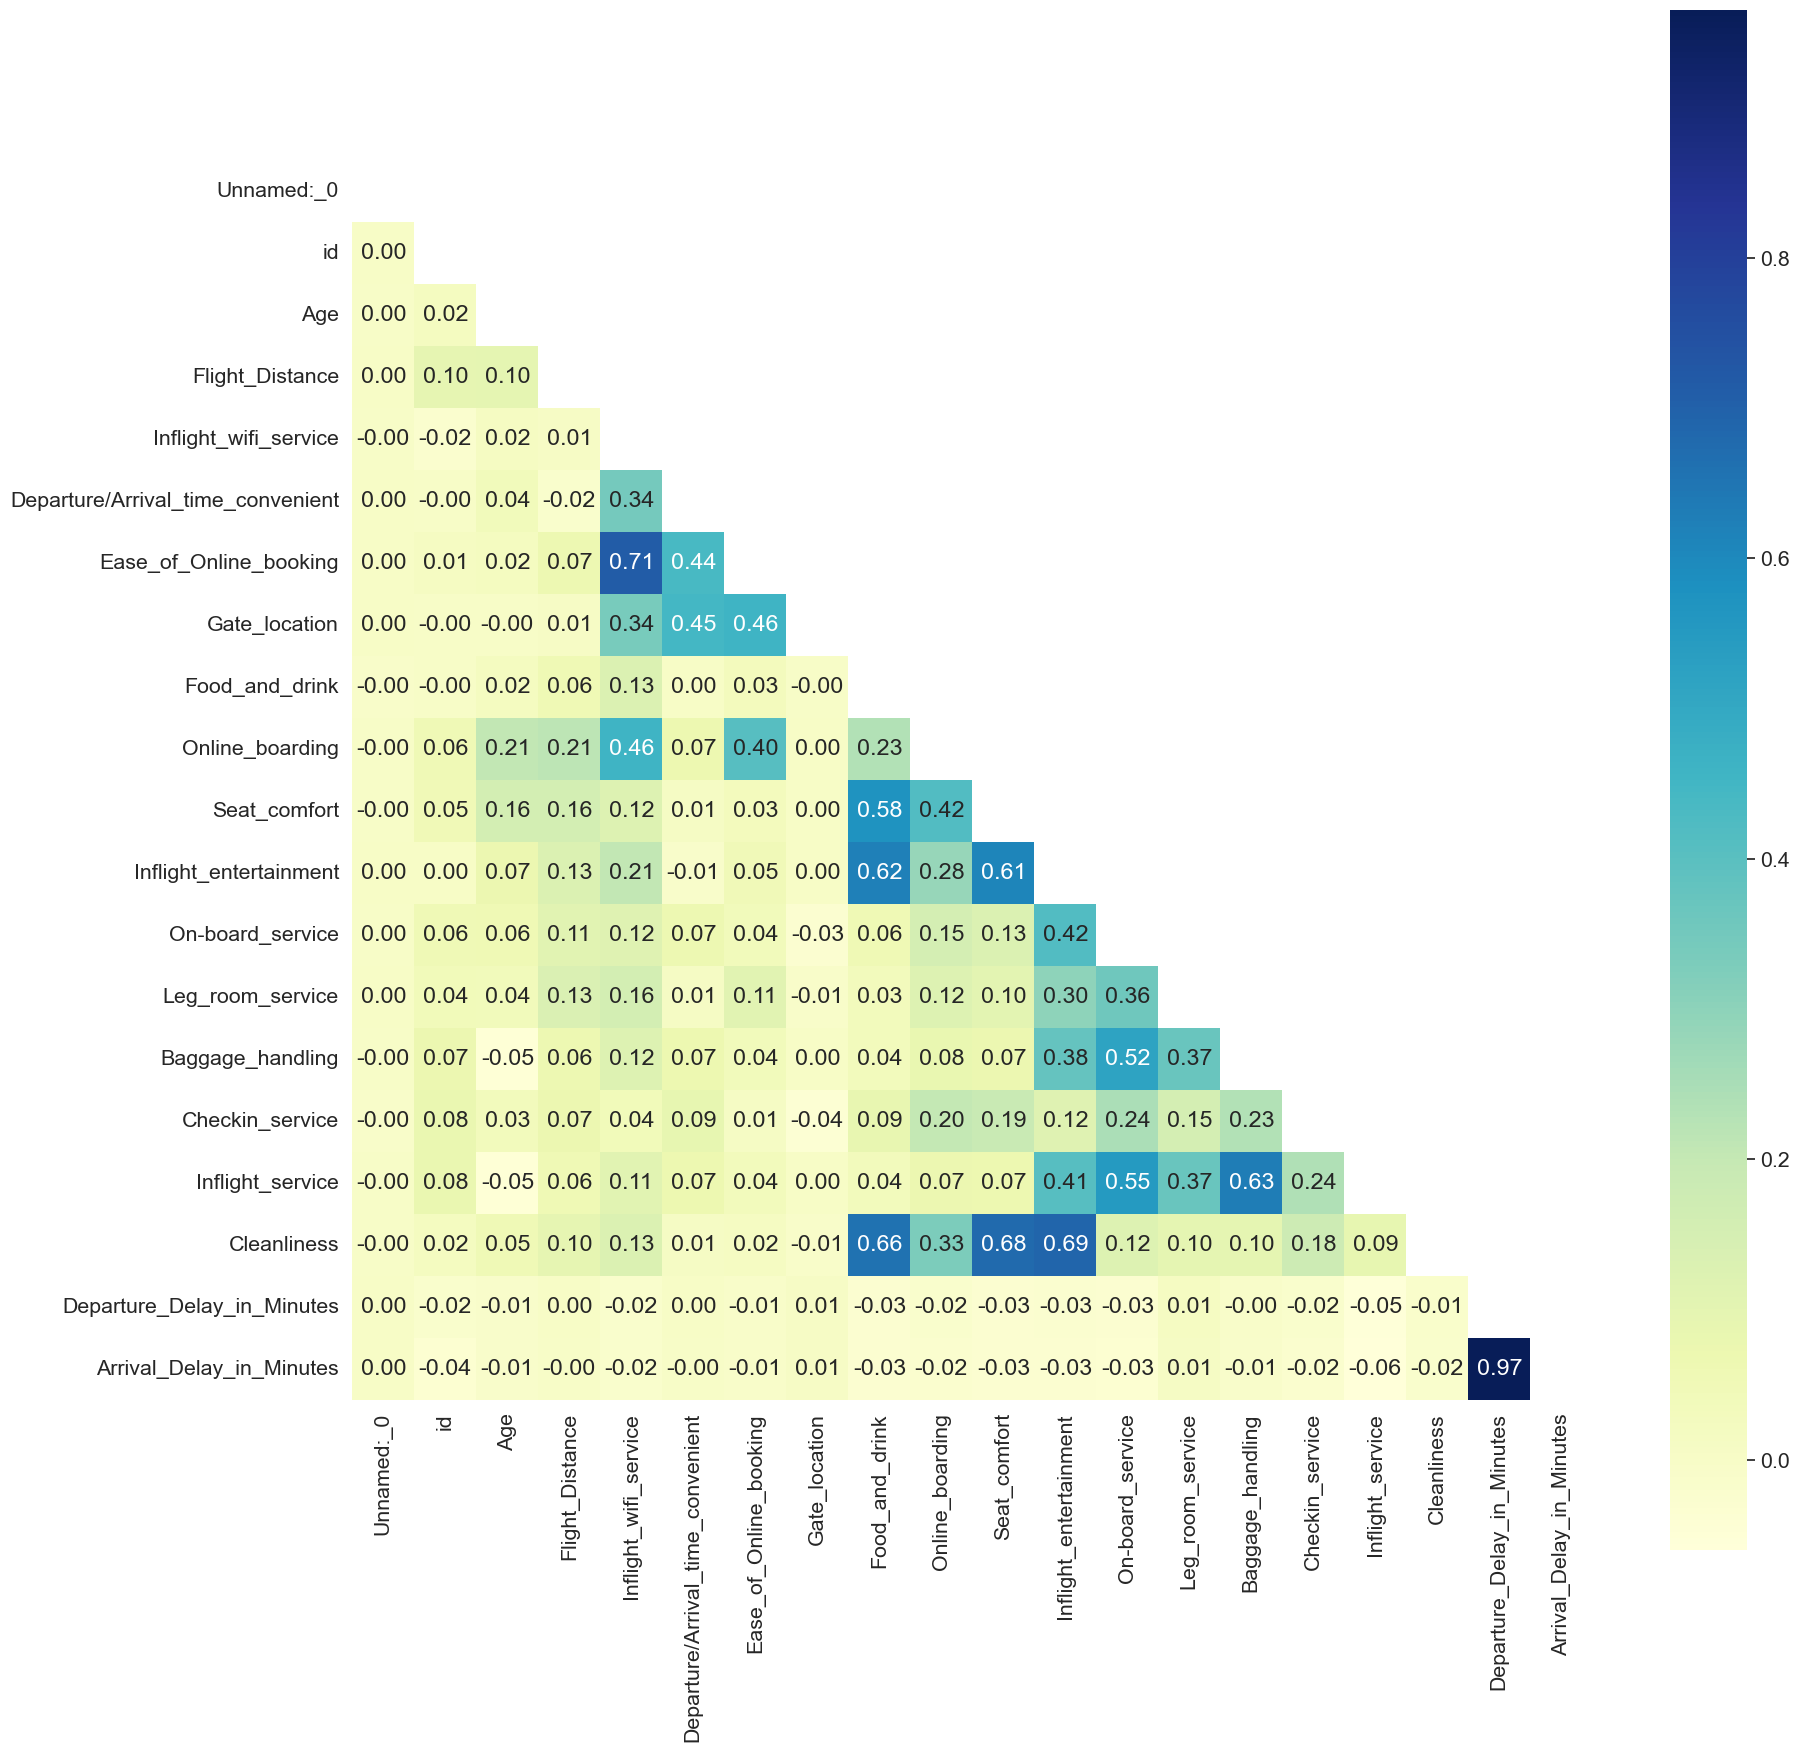
\includegraphics[width=0.8\textwidth]{images_stats/heatmap_plot.png}
    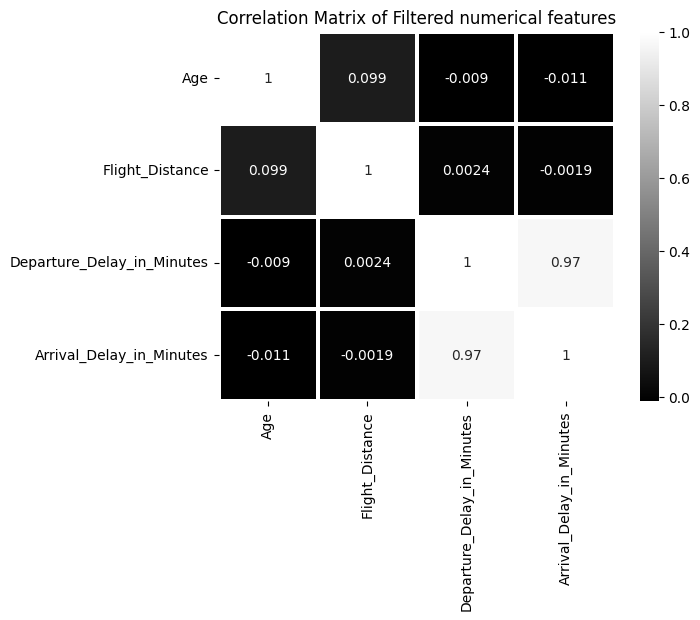
\includegraphics[width=0.8\textwidth]{images_stats/hm_numerical.png}
  \caption{Example Image}
  \label{fig:example}
\end{figure}


  
\vspace{1cm}
Inflight\_wifi\_service is very correlated with Ease\_of\_Online\_booking.
The ratings for Cleanliness are also correlated to the ratings of Food\_and\_drink, Seat\_Comfort, and Inflight\_entertainment. But the two features that are highly correlated are the Departure\_Delay\_in\_Minutes and the Arrival\_Delay\_in\_Minutes, which is very obvious, logically speaking. And we will see later on that most of our machine learning algorithms will handle this multicollinearity by applying regularized methods.



\subsection{Univariate Analysis}
In this section, we will plot each feature with respect to its frequency. Pie charts have been selected as the plotting method. Here are some figures.
\begin{figure}
  \centering
  
  \begin{subfigure}{0.45\textwidth}
    \centering
    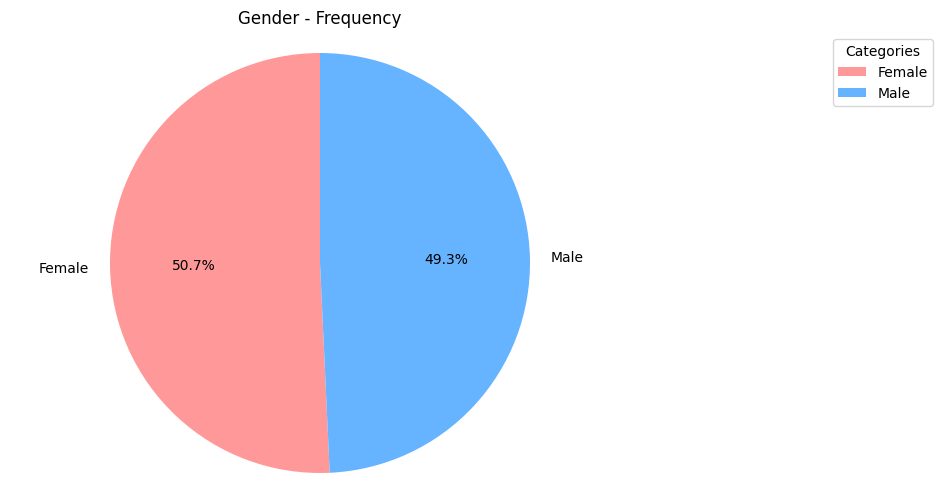
\includegraphics[width=\linewidth]{images_stats/output1.png}
    \caption{Image 1}
    \label{fig:sub1}
  \end{subfigure}
  \hfill
  \begin{subfigure}{0.45\textwidth}
    \centering
    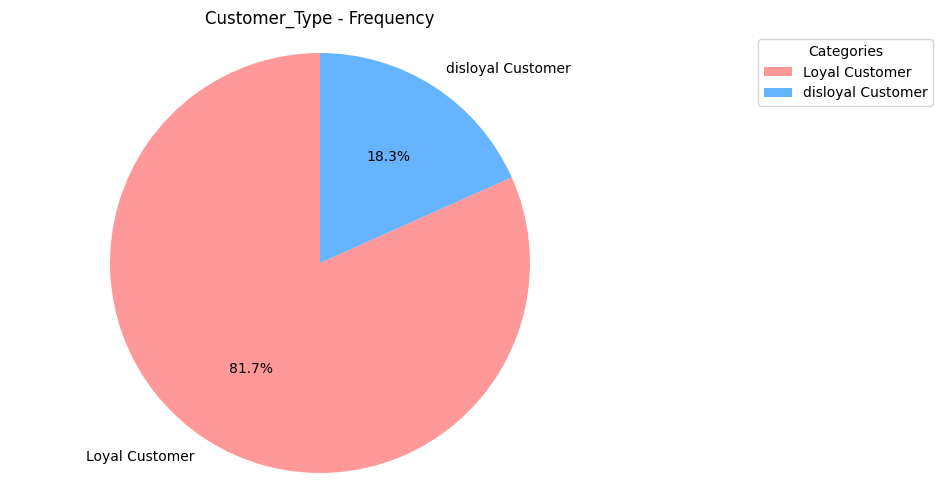
\includegraphics[width=\linewidth]{images_stats/output2.png}
    \caption{Image 2}
    \label{fig:sub2}
  \end{subfigure}
  
  \vspace{0.5cm} % Adjust the vertical spacing between rows
  
  \begin{subfigure}{0.45\textwidth}
    \centering
    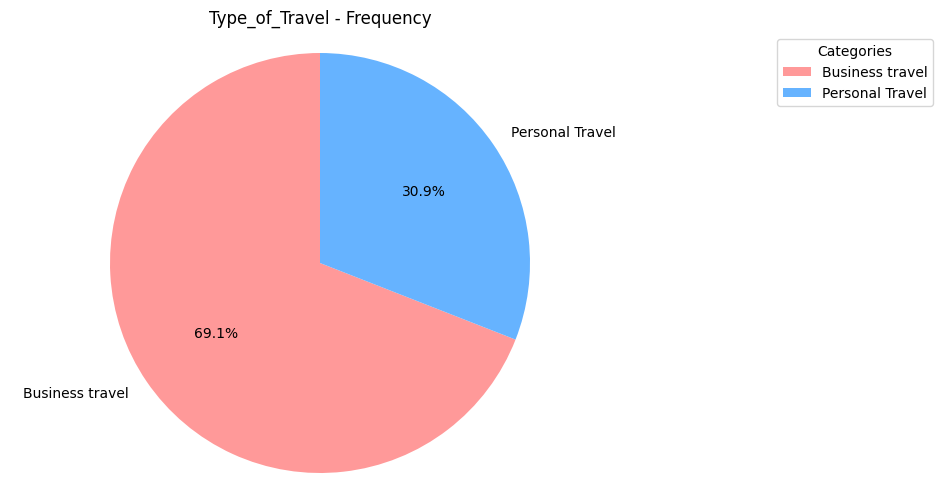
\includegraphics[width=\linewidth]{images_stats/output3.png}
    \caption{Image 3}
    \label{fig:sub3}
  \end{subfigure}
  \hfill
  \begin{subfigure}{0.45\textwidth}
    \centering
    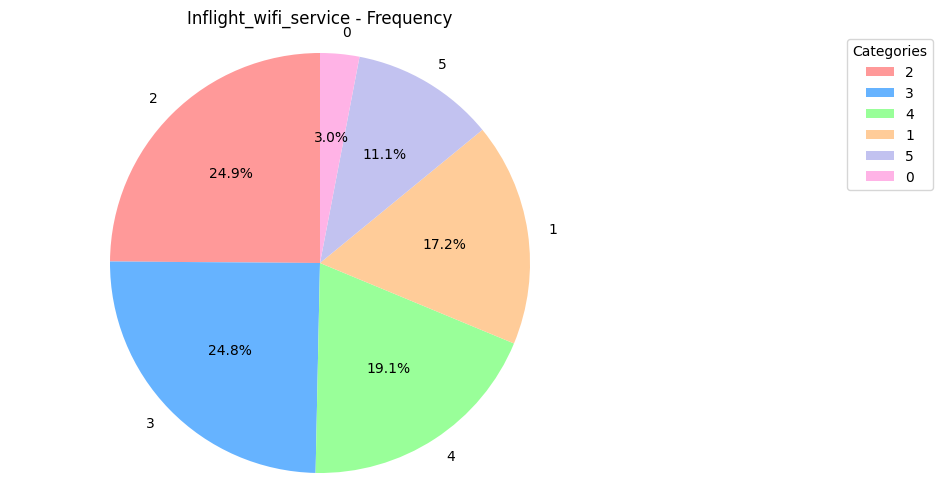
\includegraphics[width=\linewidth]{images_stats/output4.png}
    \caption{Image 4}
    \label{fig:sub4}
  \end{subfigure}
  
  \vspace{0.5cm} % Adjust the vertical spacing between rows
  
  \begin{subfigure}{0.45\textwidth}
    \centering
    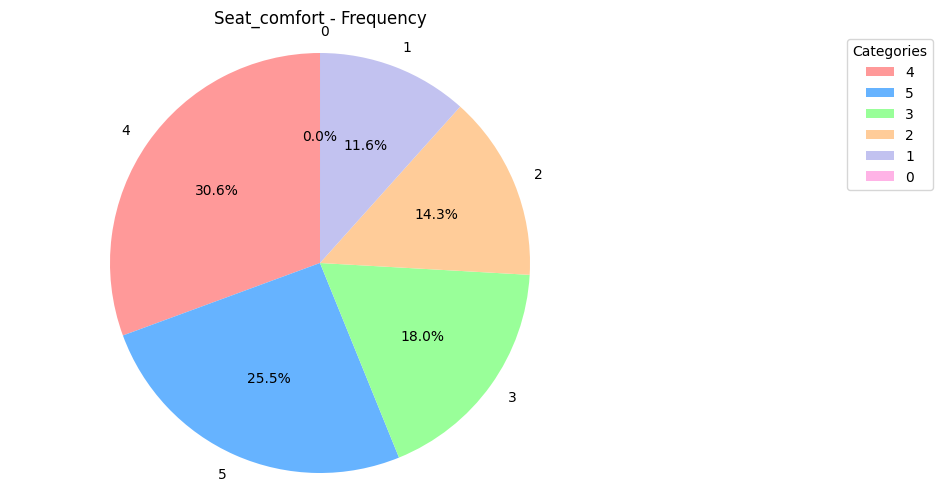
\includegraphics[width=\linewidth]{images_stats/output5.png}
    \caption{Image 5}
    \label{fig:sub5}
  \end{subfigure}
  \hfill
  \begin{subfigure}{0.45\textwidth}
    \centering
    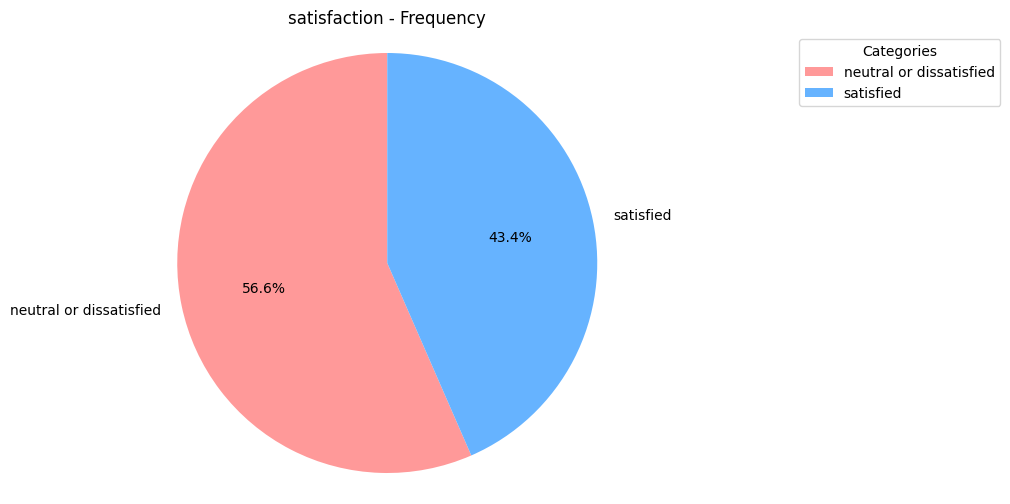
\includegraphics[width=\linewidth]{images_stats/output7.png}
    \caption{Image 6}
    \label{fig:sub6}
  \end{subfigure}

  \caption{Example Images}
  \label{fig:example}
\end{figure}








\subsection{Feature Selection}
We used 8 feature selection methods: \textbf{$\chi^2$ test, Wrapper method(random forest), decision tree and permutation importance, recursive feature elimination, backward, forward, and stepwise selection. We selected 10 features based on their importance score:}\vspace{1cm}

 \begin{enumerate}[label=\textbf{\arabic*.}]
  \item \textbf{chi\_square} = ['Customer\_Type', 'Type\_of\_Travel', 'Class', 'Inflight\_wifi\_service', 'Online\_boarding', 'Seat\_comfort', 'Inflight\_entertainment', 'On\_board\_service', 'Leg\_room\_service', 'Cleanliness']
  \item \textbf{Decision Tree} = ['Online\_boarding', 'Inflight\_wifi\_service', 'Type\_of\_Travel']
  \item \textbf{Random Forest} = ['Online\_boarding', 'Inflight\_wifi\_service', 'Type\_of\_Travel', 'Class', 'Inflight\_entertainment', 'Seat\_comfort', 'Flight\_Distance', 'Customer\_Type', 'Ease\_of\_Online\_booking', 'On\_board\_service']
  \item \textbf{Permutation} = ['Inflight\_wifi\_service', 'Type\_of\_Travel', 'Customer\_Type', 'Online\_boarding', 'Class', 'Checkin\_service', 'Seat\_comfort', 'Baggage\_handling', 'Inflight\_service', 'Cleanliness']
  \item \textbf{RFE} = ['Customer\_Type', 'Type\_of\_Travel', 'Class', 'Inflight\_wifi\_service', 'Ease\_of\_Online\_booking', 'Online\_boarding', 'On-board\_service', 'Leg\_room\_service', 'Checkin\_service', 'Cleanliness']
  \item \textbf{Backward Selection} = ['Customer\_Type', 'Type\_of\_Travel', 'Class', 'Inflight\_wifi\_service', 'Ease\_of\_Online\_booking', 'Online\_boarding', 'On-board\_service', 'Leg\_room\_service', 'Checkin\_service', 'Cleanliness']
  \item \textbf{Forward Selection} = ['Customer\_Type', 'Type\_of\_Travel', 'Inflight\_wifi\_service', 'Gate\_location', 'Online\_boarding', 'Inflight\_entertainment', 'On\_board\_service', 'Leg\_room\_service', 'Checkin\_service', 'Cleanliness']
  \item \textbf{Stepwise Selection} = ['Customer\_Type', 'Type\_of\_Travel', 'Class', 'Inflight\_wifi\_service', 'Departure/Arrival\_time\_convenient', 'Online\_boarding', 'Inflight\_entertainment', 'On-board\_service', 'Leg\_room\_service', 'Checkin\_service']
\end{enumerate}


\section{Evaluation metrics used} As for our evaluation metrics, we incorporated ROC curve, confusion matrix, and AUC(Area Under Curve). We give much emphasis on the AUC value as it will also include information about the \textbf{True Positive Rate} and \textbf{True Negative Rate}




\section{Results and Discussion} Below are the plots of the ROC curves with the mentioned evaluation metrics of our models:
\begin{figure}
  \centering
    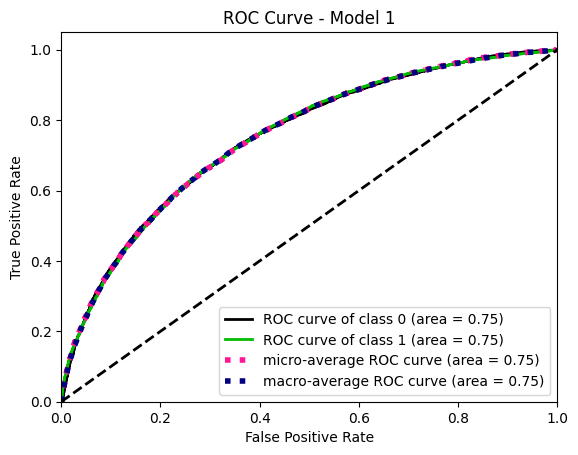
\includegraphics[width=0.8\textwidth]{images_stats/m1.png}
  \caption{Example Image}
  \label{fig:example}
\end{figure}

\begin{figure}
  \centering
    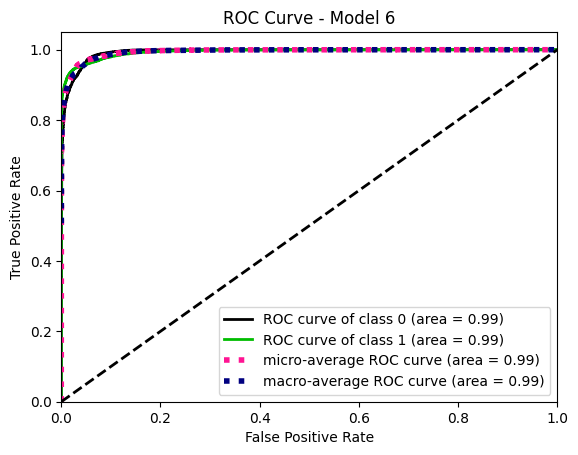
\includegraphics[width=0.8\textwidth]{images_stats/m6.png}
  \caption{Example Image}
  \label{fig:example}
\end{figure}
\begin{figure}
  \centering
    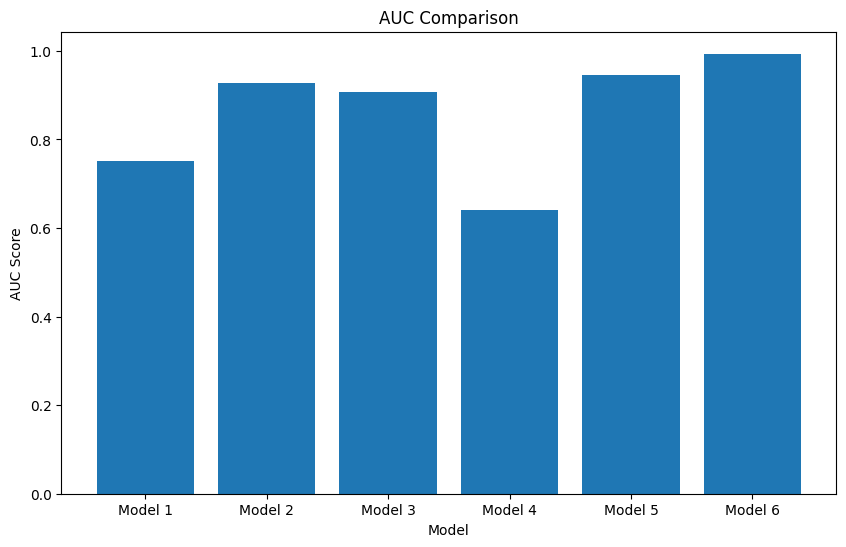
\includegraphics[width=0.8\textwidth]{images_stats/eval_scores.png}
  \caption{Example Image}
  \label{fig:example}
\end{figure}




\begin{verbatim}
Model 1: AUC = 0.7506861718066697
Model 2: AUC = 0.9267654577702052
Model 3: AUC = 0.9079386048955072
Model 4: AUC = 0.6412692385246368
Model 5: AUC = 0.9459782563100856
Model 6: AUC = 0.9935930212658386    
\end{verbatim}



\section{Conclusion} 
\textbf{In conclusion, the random forest classifier surpasses all other models in this training instance. And for important factors regarding logistic regression, we can say that ['Customer\_Type', 'Type\_of\_Travel', 'Class', 'Inflight\_wifi\_service', 'Departure/Arrival\_time\_convenient', 'Online\_boarding', 'Inflight\_entertainment', 'On\_board\_service', 'Leg\_room\_service', 'Checkin\_service'] are the most important factors in predicting airline customers' satisfaction]}

\section{Further work}
We can certainly create pipelines to ease the process and reduce time to rewrite code. We can also tune the hyper-parameter(meta-parameter) of our regularized methods. We can also train more machine learning algorithms such as Ada Gradient Boosting which is a famous and powerful classification model.

\section{Source code}



% \begin{thebibliography}{9}
% % You are free to use whatever reference style you prefer (Harvard, APA, Vancouver, etc.), but be consistent, i.e., always use the same reference style across the whole paper.
% \bibitem{} Background on logistic regression\textcolor{red}{{\url{https://en.wikipedia.org/wiki/Logistic_regression}}}
% \bibitem{} Development and history, \textcolor{red}{{\url{https://vsae.nl/nl/studenten/aenorm/2019-04-29-the-origin-of-statistics##:~:text=The\%20word\%20statistics\%20is\%20derived,agriculture\%2C\%20population\%20and\%20their\%20military.}}}
% \bibitem{} How does machine learn... \textcolor{red}{{\url{https://www.cs.cmu.edu/~avrim/Talks/mlt.pdf}}}
% \bibitem{} Some fundamentals in the theory of Statistics \textcolor{red}{{\url{https://en.wikipedia.org/wiki/Statistical_theory##:~:text=Statistical\%20theory\%20provides\%20the\%20basis,Testing\%20statistical\%20hypotheses}}}
% \bibitem{} Sourced from MIT \textcolor{red}{{\url{https://ocw.mit.edu/courses/18-650-statistics-for-applications-fall-2016/pages/lecture-slides/}}}


% \end{thebibliography}


\end{document}

